\documentclass[11pt, a4paper]{scrartcl}

\usepackage[left=3cm, right=3cm, top=3cm, bottom=3cm]{geometry}
\usepackage{graphicx}
\usepackage{array}

\newcommand{\mod}{\ \mathrm{mod} \ }
\newcommand{\git}{\mathbin{
  \mathchoice{/\mkern-6mu/}% \displaystyle
    {/\mkern-6mu/}% \textstyle
    {/\mkern-5mu/}% \scriptstyle
    {/\mkern-5mu/}}}% \scriptscriptstyle


\title{Monte Carlo Methods - Sheet 2}
\subtitle{Ising Model: Sample generation with the Metropolis algorithm}
\author{Tobias Sizmann}

\begin{document}
\maketitle
\textit{The Ising model was created by Friedrich Lenz and Ernst Ising and named after the ladder. Ising only considered a one dimensional chain of spins which does not exhibit ferromagnetism. Therefore Ising drew the conclusion that the model is not suited to explain this phenomenon. Since Ising was jewish he was arrested by Nazis in 1940 and forced to hard labor. It was only after the war that Ising found out about the success of his model. He went on to become professor for physics at the Bradley University in Illinois.}
\section{Introduction}
Due to the convergence properties Monte-Carlo methods have been proven very useful in estimating high-dimensional integrals and sums. Common discretising integrators tend to fail at high dimensions because the number of volume elements to be calculated and the resulting number of calculation steps $N$ for a fixed allowed error of estimate $\epsilon$ increases exponentially with the dimension $d$, i.e. $\epsilon = \alpha N^d$. Monte Carlo methods always converge with $\epsilon = \alpha N^{-1/2}$. It should be noted, that for most problems $\alpha$ is so large, that a Monte-Carlo approach is not feasable. Only when importance sampling is possible $\alpha$ can be small enough. Usually, importance sampling is enabled through an exponential factor in the sum or integral.

Expectation values of a Boltzmann distribution $\sum_i f(i) e^{-\beta E_i}$ in the case of the Ising model suffer a similar illness. The configuration space to be summed over increases exponentially with the number of spin sites. Therefore, small volumes of 100 spin sites are already out of reach of a straight forward numerical caluclation. The Boltzmann factor, however, weights only few configurations with a decently non-zero factor. This enables importance sampling and allows construction of a sample generation algorithm such that $\alpha$ is feasably small. Such an algorithm is the Metropolis algorithm. It allows generation of a Markov chain distributed according to the Boltzmann weights $\exp{-\beta E_i}$. In the following we will implement this algorithm for a 2D finite quadratic Ising model with periodic boundary conditions.

\section{Configuration space and grid layout}
The first task will be to find a suitable way to describe configurations. The initial idea is straight forward: Since we are considering a 2D quadratic grid of spins, a configuration may be described by a 2D matrix with entries {1, -1} representing spin up or down. Matrices must be flattened to 1D on the memory and to this end one can use the row-major memory layout. In the following $i$ denotes an index of the flattened matrix representation and $x$, $y$ of the 2D matrix. With $L$ being the extend of the grid and $\git$ being integer division, one gets the following transformations between the flattened and 2D representation:
$$
i = yL + x
$$
$$
x = i \mod L \ \ \ \mathrm{and} \ \ \ y = i \git L
$$
This construction allows us to represent a configuration in memory. Since the Hamiltonian of the Ising model depends heavily on nearest neighbor interaction it is reasonable to create a lookup table $i \rightarrow {i_{\mathrm{top}}, i_{\mathrm{right}}, i_{\mathrm{bottom}}, i_{\mathrm{left}}}$ to quickly access nearest neighbors of site $i$. With the prior transformations this can be done in a simple manner. First transform $i$ to $(x,y)$, then calculate the nearest neighbors of site $(x,y)$ according to:
$$
(x,y)_{\mathrm{top}} = (x, (y+L-1) \mod L)
$$
$$
(x,y)_{\mathrm{bottom}} = (x, (y+1) \mod L)
$$
$$
(x,y)_{\mathrm{left}} = ((x+L-1) \mod L, y)
$$
$$
(x,y)_{\mathrm{right}} = ((x+1) \mod L, y)
$$
which respects the periodic boundary conditions. Finally, transform back to the flattened representation. Such a lookup table speeds up sample generation quite a lot in contrast to calculation on the fly, since for each Metropolis sweep neighbors have to be accessed $4 L^2$ times.

\section{Measurements}
Since the memory layout of a configuration has been dealt with, the next step is to implement measurements on such a configuration. In particular, we are interested in energy and magnetisation density. Interestingly we will see that the change in both these quantities can be calculated very efficently during the Metropolis steps. Therefore, an absolute measurement of energy and magnetisation will only be required for initialising these values. For a configuration $c$ in flattened representation, these are given by
$$
e(c) = \frac{1}{L^2}\sum_i ( c(i)c(i_{\mathrm{right}}) + c(i)c(i_{\mathrm{bottom}})
$$
$$
m(c) = \frac{1}{L^2} \sum_i c(i)
$$
Two remarks are necessary here. First, for the energy only the interaction with two neighbors must be considered, since the interactions in the other directions are dealt with by other center sites. Secondly, we are not yet considering the absolute value of the magnetisation. Otherwise the performance enhancing trick would not work. It is important to note that statistical momenta like the mean should always be calculated over the absolute value of the magnetisation to have a physical interpretation.

\section{Metropolis algorithm}
The Metropolis algorithm builds the Markov chain. It works in the following way:
\begin{itemize}
\item[1. ] Consider the last configuration in the Markov chain $c$ and a site $i$. Calculate the energy difference $\Delta E = E_{\mathrm{New}} - E_{\mathrm{Old}}$ if one would switch the spin on this site. One can quickly see, that $\Delta E$ only takes the values -8, -4, 0, 4, 8.
\item[2. ] Calculate $p = e^{- \beta\,\Delta E}$. This can be sped up by creating a lookup table for the five possible values of $\Delta E$. Draw a random number $d$ uniformly distributed from 0 to 1.
    \begin{itemize}
    \item If $d < p$ then reject the change by adding a copy of the prior configuration to the Markov chain: $c_{\mathrm{next}} = c$.
    \item If $d > p$ then accept the change by adding a copy of the prior configuration to the Markov chain but with flipped spin on site $i$: $c_{\mathrm{next}} = c$ and $c_{\mathrm{next}}(i) *= -1$ The new energy is then $e += \Delta E/L^2$ and the new magnetisation is $m += -2c(i)/L^2$
    \end{itemize}
\end{itemize}
Since the resulting chains for energy and magnetisation are the only quantities we are interested in, the prior configuration $c$ can be discarded and only the new configuration $c_{\mathrm{next}}$ must be saved for the next Metropolis step. One can save the magnetisation state internally and append the absolute value to the chain. One sweeps through ever site of the grid before visiting the first one again.

\section{Specific heat and magnetic susceptibility}
After a chain has been generated and thermalized, one can compute second order quantities like specific heat and magnetic susceptibility. In the following $t_M$ denotes the Markov time and $e(t_M)$ and $m(t_M)$ the energy density and absolute magnetisation density at this time step. The specific heat density $c$ and magnetic susceptibility density $\chi$ are then given by:
$$
c = \frac{\beta ^ 2}{L^2} (\langle E^2 \rangle - \langle E \rangle ^ 2) = \beta ^ 2 L^2 (\langle e^2 \rangle - \langle e \rangle ^ 2)
$$
$$
\chi = \frac{\beta}{L^2} (\langle M^2 \rangle - \langle M \rangle ^ 2) = \beta L^2 (\langle m^2 \rangle - \langle m \rangle ^ 2)
$$
Note that for density quantities depending on variances of density quantities an additional $L^2$ must be introduced to compensate for the $L^{-4}$ factor emerging from the variance.

\section{Results}
\subsection{Sample generation and thermalisation}
\begin{figure}
    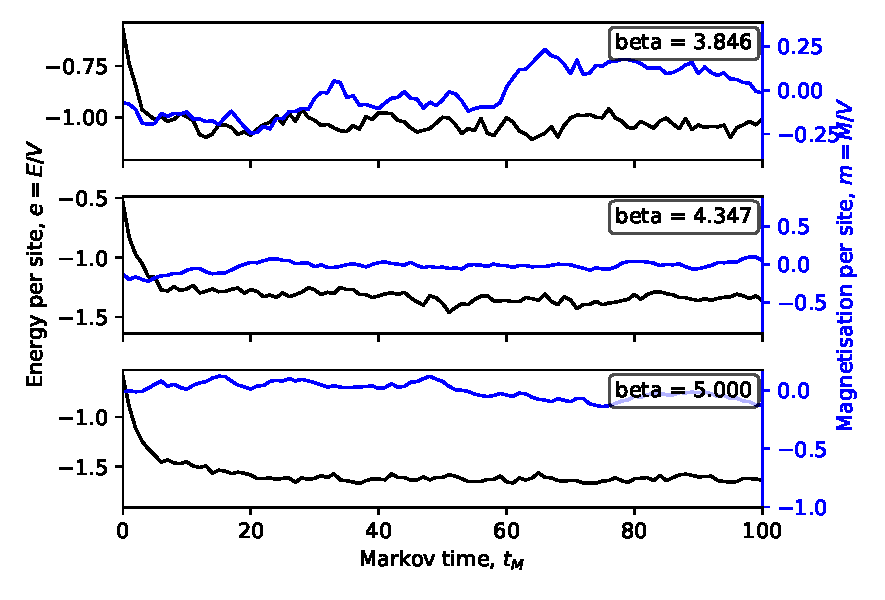
\includegraphics{chains_therm.pdf}
    \label{therm}
    \caption{\textbf{Thermalisation of Markov chains generated by the Metropolis algorithm:} Energy density $e = E/V$ (black) and absolute magnetisation density (blue) $m = \left| M \right| / V$ have been plotted for the first 100 sweeps of streams with inverse temperatures $T = 1 / \beta = 2.0, 2.3, 2.6$. The thermalisation process in energy is recognizable by the (roughly) exponential decay at the beginning and discarding the first 50 values is a safe choice. We will see, however, that for $\beta = 0.5$ this is a false choice. For the magnetisation densities the thermalization is not so clear at all. The chains are also plotted for the first 10000 sweeps in fig. \ref{10000} where a sensible choice of thermalisation for the magnetisation density can be made.}
\end{figure}

\begin{figure}
    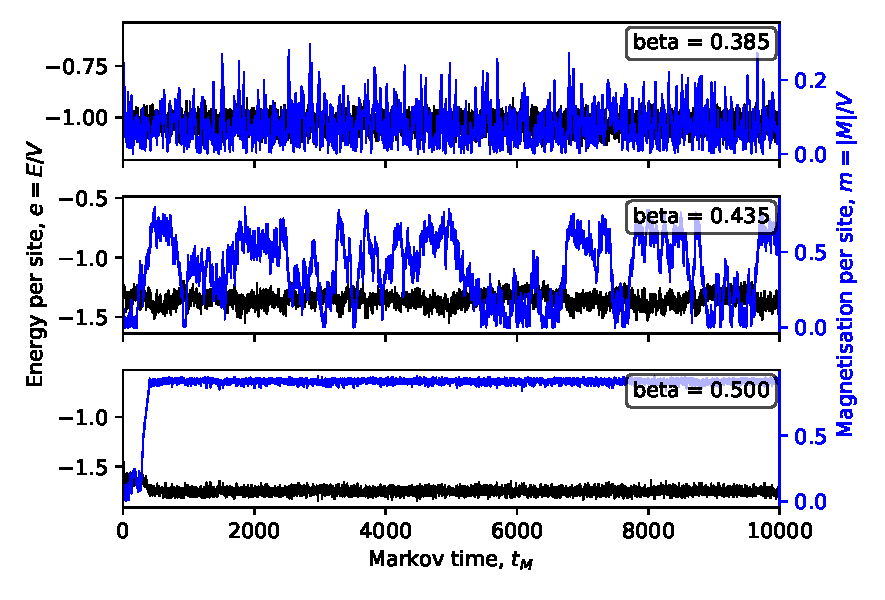
\includegraphics{chains_10000.pdf}
    \label{10000}
    \caption{\textbf{Thermalisation of Markov chains generated by the Metropolis algorithm:} Energy density $e = E/V$ (black) and absolute magnetisation density (blue) $m = \left| M \right| / V$ have been plotted for the first 10000 sweeps of streams with inverse temperatures $T = 1 / \beta = 2.0, 2.3, 2.6$. Here one sees clearly that for $\beta = 0.5$ the system takes about 500 steps to fully thermalise.}
\end{figure}

We now want to test how the indroduced concepts work out in practice. To this end three streams with grid size $L = 64$ and temperatures $T = 2.0, 2.3, 2.6$ have been generated each with $N = 100000$ Metropolis sweeps. The energy densities and magnetisation densities have been saved and are plotted for the first 100 sweeps in fig. \ref{therm} and for the first 10000 sweeps in fig. \ref{10000}. The plots can be used to make sensible choices for thermalisation of both the energy density and magnetisation density. It should be noted that sample generation for the Ising model is very cheap and therefore the thermalisation cutoff can be choosen generously. The plots in Fig. \ref{therm} for the energy suggest to discard the first 50 values. We will see that for $\beta = 0.5$ this has to be corrected. The situation for the magnetisation is a bit more involved (see fig. \ref{10000}). For the $T=2.6$ stream (i.e. $\beta = 0.385$) thermalisation is not noticable and therefore it is reasonable to choose a cutoff in the order of the resolution of the plot (here about 100 steps). For the $T=2.3$ stream (i.e. $\beta = 0.435$) a decision on the thermalisation cutoff is hard since the autocorrelation is so large. Still one might say that the short plateau at the beginning might be due to thermalisation. Therefore we will choose a cutoff of 1000 steps which is well beyond this plateau. The $T=2.6$ stream (i.e. $\beta = 0.5$) is particularly interesting. One can see that thermalisation takes place in two steps. First the immediate thermalisation within 20 steps and then a second thermalisation of the magnetisation. This could have been avoided by choosing a better initial configuration, which already has a majority of spins up or down. In the following the first 1000 steps have been discarded of this stream.

\subsection{Measurements}
After thermalisation of the streams, one can calculate physical quantities of interest. Namely, mean energy, mean magnetisation, specific heat and magnetic susceptibility. The calculations according the formulas established earlier are straight forward and the results are presented in the table below:
\begin{center}
\begin{tabular}{ | m{2cm} || m{2cm}| m{2cm} | m{2cm} | m{2cm} | }
  \hline
  Temp. $T$ & $\langle e \rangle$ & $\langle m \rangle$ & $c$ & $\chi$\\
  \hline
  2.6 & -1.03 & 0.075 & 0.708 & 4.886\\
  \hline
  2.3 & -1.355 & 0.425 & 2.159 & 72.994\\
  \hline
  2.0 & -1.745 & 0.911 & 0.729 & 0.388 \\
  \hline
\end{tabular}
\end{center}
No errors are calculated on these values so far, so the following physical interpretation should be taken with reserve. One can see that the energy increases and the magnetisation decreases with temperature. Interestingly the susceptibilities of energy and magnetisation seem to diverge close to $T = 2.3$. This is very close to the critical temperature and susceptibilities are expected to diverge logarimically here. Therefore, one can conlude that the Monte Carlo approach allows us to at least display the most important physical properties. An exact quantitative discussion can be done, when errors are calculated. 
\end{document}
